\documentclass[letterpaper,12pt]{article} %tipo de documento y tama~o de papel y letra
\usepackage[latin1]{inputenc} %codificacion de caracteres
\usepackage[spanish]{babel} %idioma
\usepackage{fancyhdr} %tipo de pagina, LINDA biggrin.gif
\usepackage[top=3.5cm,bottom=2.5cm,right=2cm,left=2.5cm]{geometry} %margenes
\usepackage[rflt]{floatflt} %ni puta idea
\usepackage{pdfpages} %incluir archivos pdf
\usepackage{float}
\usepackage{hyperref} %hipervinculos
\hypersetup{
  colorlinks=true,
  urlcolor=cyan
}
%\usepackage{helvet} %esto es pa escribir con Arial en vez de times new roman
%\renewcommand\familydefault{\sfdefault} %descomenta estas lineas para escribir en arial

\usepackage{multirow}

\usepackage{graphicx} %para usar imagenes
%\newcommand{\imgdir}{doc-img} % para meter las imagenes en una carpeta especial, tunz en la carpeta del documento tiene q ir otra que se llame 'doc-img'
\graphicspath{{./pic/}} %le dice que las imagenes estan en la carpeta de arriba

\usepackage{amsmath} %pa usar smbolos matematicos
\numberwithin{equation}{section} % pa usar ecuaciones de modo lindo
\numberwithin{figure}{section} %para agregar imagenes
\numberwithin{table}{section} %para agregar tablas

\usepackage{chngcntr}
\counterwithin{equation}{section}
\counterwithin{figure}{section}
\counterwithin{table}{section}

\usepackage{subfigure} % pa usar sub figuras



\pagestyle{fancy} %configuracion para la pagina linda
\renewcommand{\sectionmark}[1]{\markboth{}{\thesection\ \ #1}} %cambios de comentarios
\lhead{} %parte de arriba, izq
\chead{} %parte de arriba, centro
\rhead{\rightmark} %parte de arriba, derecha, le agrega la marca del capitulo
\lfoot{} %parte de abajo, izq
\cfoot{} %parte de abajo, centro
\rfoot{\thepage} %parte de abajo, derecha, va el numero de la pagina


%-------------portada---------------------------------%
\begin{document}
\begin{titlepage} %portada
\thispagestyle{empty} %borrar el formato de pagina linda
%\begin{flushleft} %alinear a la izq
\begin{center}

\includegraphics[scale=0.35]{logoUSM-DI.eps}
%\vfill
\end{center}
%\end{flushleft}

\vspace{3cm} %espacio vertical , en realidad es un enter de 2 cm
\begin{center} %centrar
  {
    \Huge Artefactos de Mitigaci\'on\\
    \huge Proyecto ``\emph{V.I.Pe.R.}''\\
    \normalsize\today
  }
\end{center}

\vspace{6cm}

\vfill
\begin{flushleft} %alinear derecha
Pre-Empresa: \emph{Phyrex}\\
Jefe de Proyecto: Rodrigo Fr\'{\i}as\\
Integrantes:
\begin{table}[hb]
  \begin{tabular}{lcc}
    Rodrigo Fr\'{\i}as & \texttt{\small <rodrigo.frias@alumnos.usm.cl>} & [+56 9 83988257] \\
    Celeste Bertin & \texttt{\small <celeste.bertin@alumnos.usm.cl>} &[+56 9 68410901]\\
    Patricio Carrasco &\texttt{\small <patricio.carrascod@alumnos.usm.cl>} &[+56 9 50626689]\\
    Rocio Fernandez &\texttt{\small <rocio.fernandezu@alumnos.usm.cl>} & [+56 9 62426549]\\
    Juan Avalo & \texttt{\small <juan.avalo@alumnos.usm.cl>} & [+56 9 78072458]\\
  \end{tabular}
\end{table}
\end{flushleft}
\end{titlepage}
%------------------fin de la portada --------------------%

%{\bf } %escribir en negrita

\setcounter{page}{1} %empezar enumerando la pagina 1

%\tableofcontents

%\newpage
\section{Artefactos de Mitigaci\'on.}
Para mitigar nuestro principal riesgo (a saber, \emph{Errores de inicio y mantenci\'on de conexi\'on v\'ia Bluetooth entre aplicaci\'on y sistema rob\'otico}) fue utilizado:

\begin{itemize}
\item Robot con un NXT Intelligent Brick y 3 motores.
\item Aplicaci\'on Android de control.
\end{itemize}

%\newpage
\section{C\'odigo Desarrollado.}
Para resolver nuestro principal riesgo, se desarroll\'o una aplicaci\'on Android con la capacidad de conectarse con los NXT Intelligent Brick, el cual utiliza la librer\'ia ``BluetoohAdapter'' de las librerias de Bluetooth de Android.

De ella, la aplicaci\'on desarrollada utiliza las siguientes funciones, para mantener la conexi\'on entre el dispositivo m\'ovil (smartphone) y el Robot.

\begin{itemize}
\item {\bf \verb+createBTCommunicator()+}: crea objeto para realizar conexi\'on
\item {\bf \verb+startBTCommunicator()+}: inicia la conexi\'on
\item {\bf \verb+destroyBTCommunicator()+}: termina la conexi\'on
\end{itemize}

Es a trav\'es de dichas funciones, que el dispositivo es capaz de mandarle las instrucciones necesarias al robot (por medio del NXT Intelligent Brick) para poder mover sus motores.

%\newpage
\section{Relaci\'on Entre Elementos.} %1 pag
Para poder observar la relaci\'on existente entre los distintos elementos que interact\'uan con el sistema, se adjunta el diagrama de secuencia, observable en la Figura~\ref{img:diagrama}, en donde se detalla el funcionamiento de la soluci\'on implementada para mitigar el principal riesgo.

\begin{figure}[H]
   \centering
     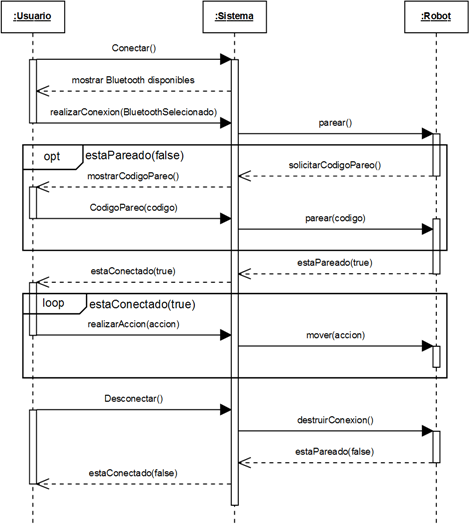
\includegraphics[scale=1]{DiagramaSecuencia_v01.png}
   \caption{Diagrama de Secuencia de funcionamiento del Demo realizado para la mitigaci\'on del riesgo principal.}
   \label{img:diagrama}
\end{figure}


\end{document}

%%%%%%%%%%%%%%%%%%%%%%%%%%%%%%%%%%%%%%%%%%%%%%%%%%%%%%%%%%%%%%%%%%%%%%%%%%%%%%%%
%\begin{figure}[H]
%   \centering
%     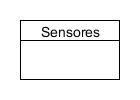
\includegraphics[scale=0.45]{ModeloDominio.jpg}
%   \caption{Se puede apreciar el Modelo de Dominio relativo a \emph{V.I.Pe.R}.}
%   \label{fig:ModeloDominio}
%\end{figure}
%%%%%%%%%%%%%%%%%%%%%%%%%%%%%%%%%%%%%%%%%%%%%%%%%%%%%%%%%%%%%%%%%%%%%%%%%%%%%%%%
%\begin{table}[H]
%  \centering
%  \begin{tabular}{p{5cm}p{9cm}}\hline
%    Entidad & Descripci\'on \\ \hline \hline %1 linea
%    Usuario & Representa a quien va a ocupar la aplicaci\'on (Un alumno, por ejemplo). \\ \hline
%    Encargado & Es el que se encarga de mantener al robot y obtener los datos necesarios para difusion. \\ \hline
%    Smartphone & Maneja las interacciones entre el usuario y la mascota. Debe tener SO Android. \\ \hline
%    Mascota Virtual & Representa el ``cerebro'' de la mascota. \\ \hline
%    Robot & Es el robot f\'isico, con las capacidades que tienen que estar almacenadas si o si en \'el. \\ \hline
%    Motores & Representa a los motores que permiten que el robot se mueva. \\ \hline
%    Brick & Representa a la unidad de control del robot. \\ \hline
%    Sensores & Representan a los sensores que puede poseer el robot y que le permiten obtener informacion del ambiente. \\ \hline \hline
%  \end{tabular}
%\end{table}
%%%%%%%%%%%%%%%%%%%%%%%%%%%%%%%%%%%%%%%%%%%%%%%%%%%%%%%%%%%%%%%%%%%%%%%%%%%%%%%%
